\documentclass[sigconf,anonymous,review]{acmart}
\usepackage{amsmath,booktabs,graphicx}
\setlength{\emergencystretch}{1em}
\setcopyright{none}
\settopmatter{printacmref=false}
\acmConference[WWW '27 submission]{The ACM Web Conference}{2027}{Dublin, Ireland}
\acmYear{2027}
\acmDOI{}\acmISBN{}
\renewcommand\footnotetextcopyrightpermission[1]{}
\title{Evaluating Predictive Models and AI Agents for Blockchain Oracle Adjudication}
% Generated from completed saved predictions; do not edit numeric claims manually.
\newcommand{\AbstractAblation}{Fresh predictor removal increases planner Brier by $+0.0846$ (95\% CI $[+0.0479,+0.1225]$).}
\newcommand{\AblationFinding}{Fresh removal changes A1 Brier by $+0.0846$ (95\% CI $[+0.0479,+0.1225]$) and A2 by $+0.0831$ (95\% CI $[+0.0473,+0.1197]$). This tests access to the predictor, including the induced change in tool policy. Fresh A1 controls call $B^\star$ in 470/471 trajectories, versus none without access. Across repeats, A1 Brier ranges from 0.2348 to 0.2365 with access and 0.2911 to 0.3509 without it.}
\newcommand{\VerificationFinding}{In fresh controls, 7/471 outputs change (3 improve, 4 worsen), with A2--A1 $+0.00033$ (95\% CI $[-0.00008,+0.00092]$); without the predictor, 16/471 change (7 improve, 9 worsen), with $-0.00120$ (95\% CI $[-0.00722,+0.00406]$). Of these, 1 change involves a prior fallback (marked in Figure~\ref{fig:results}D); trace analysis separates fallback from valid revisions.}
\newcommand{\TemporalFinding}{All six calendar-block intervals for predictor removal remain above zero.}
\newcommand{\ExecutionFinding}{The fresh ablation uses 3,463 calls with 0 transport failures and 5 fallback outputs across 1,884 predictions; its inference allocation is 14.35 GPU-hours.}
\newcommand{\PreparationFinding}{A separate exact replay of shared offline preparation takes 9.41\,s; fresh $B^\star$ warm service takes 140.99\,ms median, including packet preparation.}
\newcommand{\ConclusionAblation}{The access intervention supports dependence on the conventional predictor; these results do not establish an orchestration advantage beyond that predictor.}

\begin{document}
\begin{abstract}
Do planning and verification improve oracle forecasts beyond the predictor and evidence they use? We evaluate this question on released UMA data, predicting eventual protocol disagreement from proposal-time inputs. A chronological, question-disjoint evaluation retains 474 training, 153 validation and 157 test requests. Conventional predictors are compared with a shared-backbone direct LLM, tool planner, verifier and matched-evidence control. In the original comparison, the verifier obtains Brier 0.2360 versus 0.2355 for the validation-selected ensemble: paired difference $+0.0005$ (95\% CI $[-0.0008,0.0017]$). Verification changes eight of 471 repeated predictions, helping four and harming four. \AbstractAblation{} We report question-cluster uncertainty, temporal sensitivity and measured latency. These exploratory comparisons concern a retrospectively selected disputed cohort and protocol outcomes, not external factual truth or population-wide risk.
\end{abstract}
\ccsdesc[500]{Computing methodologies~Machine learning}
\keywords{blockchain oracles, agent evaluation, probabilistic prediction, temporal evaluation, predictor attribution}
\maketitle
\raggedbottom

\section{Introduction and related work}
Blockchain oracles connect Web information to application settlement. Optimistic protocols let participants propose an outcome, challenge it and obtain a later adjudication. Forecasting that adjudication is distinct from establishing whether a real-world claim is true. Agents that plan tool use and verify a draft may help, but an apparent gain can originate from the conventional predictor they call.

Prior oracle work already uses web-enabled LLMs to reproduce UMA resolutions after a dispute and predicts dispute formation from event rules~\cite{wen2026}. Our narrower question is whether orchestration adds predictive value beyond a fitted predictor and matched evidence under a proposal-time cutoff. We study structured event histories, not semantic fact checking; these tasks and scores are not interchangeable. We reuse the released Atlas resource~\cite{Jia2026OracleAtlas}, making no new-dataset or first-LLM claim.

Zhu et al.~\cite{zhu2025} distinguish task validity from outcome validity; we accordingly define the information boundary and avoid equating protocol agreement with truth. Kapoor et al.~\cite{kapoor2025} motivate attribution controls, honest holdouts and joint accuracy--cost reporting. TabArena~\cite{erickson2025tabarena} motivates validation-based tuning and ensembling, while our temporal grouping replaces its IID setting. TabPFN's small-data results~\cite{hollmann2025} also caution against treating a small conventional search as a universal best baseline. We prioritize controlled attribution here and do not evaluate TabPFN.

We contribute a temporal evaluation with auditable inputs, controls for predictors and evidence, and paired uncertainty backed by execution records. Earlier experiments exposed this historical test; both the original comparison and the new access ablation are exploratory. There is no untouched later test.

\section{Task and temporal protocol}
For request $i$, proposal time $T_i$, proposed value $v_i^p$ and eventual resolved value $v_i^r$, define
\begin{equation}
\begin{aligned}
Y_i&=\mathbf1\{\operatorname{int}(v_i^r)\ne\operatorname{int}(v_i^p)\},\\
p_i&=\Pr(Y_i=1\mid X_i(T_i),T_i,S_i=1).
\end{aligned}
\end{equation}
$S_i=1$ denotes the retrospectively challenged, linked, settled and transfer-reconciled cohort. Selection partly depends on events after $T_i$; it is not an observable deployment filter. The label includes special integer outcomes such as early expiration, with variable resolution delay.

The pinned release \texttt{atlas-utc-20261029} (commit \texttt{a8e4e930}) contains 810 task requests / 623 questions. We replay published native events, without claiming an independent blockchain receipt audit. Eleven inputs survive the availability audit: log final fee in raw units, liveness, proposal latency, ancillary byte length, proposed-value class, and completed-count, dispute-rate and rejection-rate histories for proposer and requester. Four unbound parameter features and an adapter flag are excluded. Histories use 40,534 primary requests, restricted to settlements strictly preceding the proposal in $(\mathrm{UTC},\mathrm{block},\mathrm{transaction},\mathrm{log})$ order. Empty-history rates remain null; preprocessing fits training inputs only. No question text, live Web evidence or current-request outcome enters prediction.

Validation starts on 1 April 2025, 16:00:45 UTC; test starts on 1 July 2025, 03:51:31 UTC. Entire questions crossing partitions are purged (10 requests). Training and validation labels must settle before their next partition starts (another 12 and 4 requests removed). This leaves 474/153/157 requests and 367/121/120 questions, with 84 test positives. Settlement is a conservative label-availability proxy. Model weights remain fixed, while shared histories may incorporate earlier test settlements already public at $T_i$.

\begin{figure*}[t]
\centering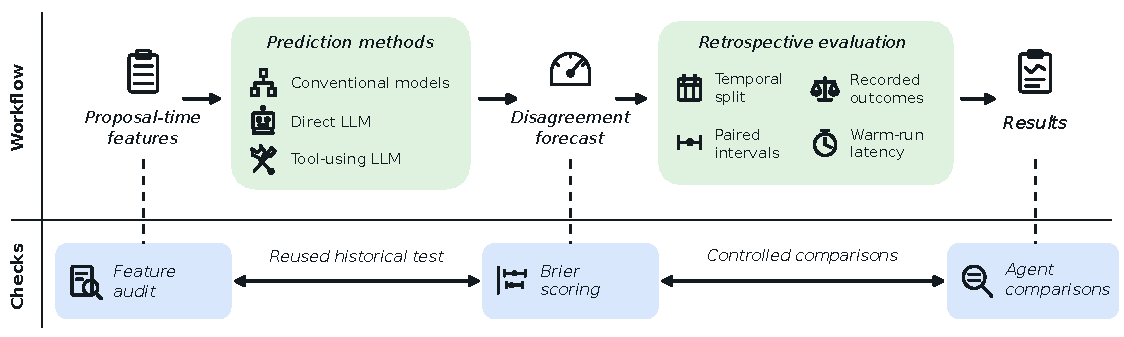
\includegraphics[width=\textwidth]{figures/method.pdf}
\caption{Executed workflow and checks for retrospective protocol-disagreement prediction. Models use proposal-time features; LLM packets also include the cutoff and training prior, with read-only tools. Recorded settlements supply scoring labels. Chronological, question-disjoint splits reuse a previously examined test set; comparisons are exploratory. The lower row names feature auditing, Brier scoring and agent comparisons; the latter test predictor access, matched evidence and verification. Dashed links associate checks with workflow stages. Paired intervals concern performance differences; latency covers warm runs. No established agent gain or external-truth validation is implied.}
\Description{A green and blue two-row diagram. The upper workflow connects proposal-time features, conventional and LLM prediction methods, disagreement forecasts, retrospective evaluation and results. Evaluation uses temporal splits, recorded outcomes, paired intervals and warm-run latency. The blue lower row contains feature audit, Brier scoring and agent comparisons, linked by reused historical test and controlled comparisons. Neutral line icons replace success markers. The diagram contains no numbers.}
\label{fig:method}
\end{figure*}

\section{Predictors and agent controls}
\paragraph{Conventional predictors.}
With $\sigma$ the logistic function, predictions are
\begin{equation}
\begin{aligned}
p_{\rm prior}&=n_{\rm tr}^{-1}\!\sum_{\rm tr}Y_i,&
p_{\rm LR}(x)&=\sigma(\beta_0+x^\top\beta),\\
p_{\rm RF}(x)&=500^{-1}\!\sum_b\hat\pi_{L_b(x)},&
p_{\rm GBM}(x)&=\sigma(F_0+.03\!\sum_m f_m(x)),\\
p_{\rm ens}(x)&=\sum_m w_mp_m(x),&w_m&\ge0,\ \sum_mw_m=1.
\end{aligned}
\end{equation}
LR uses summed log loss with penalty $\|\beta\|_2^2/(2C)$. We search $C\in\{.01,.1,1,10\}$; median imputation, missing indicators, scaling and encoding fit training data only. RF~\cite{breiman2001} uses 500 bootstrap trees, Gini splits, depth $\{4,8\}$ and leaf size $\{3,10\}$. LightGBM~\cite{ke2017} uses logistic loss, leaves $\{7,15\}$, leaf size $\{10,30\}$ and at most 1,000 rounds. AutoGluon 1.6.1~\cite{erickson2020} fits these eight tree candidates and a greedy weighted ensemble~\cite{caruana2004}. Across 14 candidates including prior and LR, validation Brier chooses $B^\star$: $6/7$ LightGBM plus $1/7$ RF. AutoML bagging, stacking, refitting and calibration are disabled; forest bootstrap remains enabled. This is a small audited search, not an unrestricted AutoML leaderboard.

\paragraph{Matched LLM systems.}
All use the same frozen Qwen3.8-27B snapshot~\cite{qwen2026} in BF16, temperature .7, top-$p$ .95, top-$k$ 20, thinking disabled and 512 output tokens per call. Their shared packet $P_i=(X_i(T_i),T_i,\hat\pi)$ exposes the cutoff timestamp and training prior alongside the 11 features. Conventional models consume $X$. D0 is $L_\theta(P)$, one direct pass. Starting from $s_0=P_i$, A1 follows a bounded tool policy~\cite{yao2023react}:
\begin{equation}
\begin{aligned}
a_k&\sim\pi_\theta(\cdot\mid s_k), & o_k&=\mathcal T(a_k;T_i),\\
s_{k+1}&=U(s_k,a_k,o_k), & p_1&=g_\theta(s_\tau).
\end{aligned}
\end{equation}
Tools return proposal inputs, existing actor histories, the exact $B^\star$ probability, bounded arithmetic or evidence-ID validation. The server fixes the case and cutoff. These histories duplicate packet information; the predictor output is the principal additional learned signal. A2 checks the same A1 draft using $z=V_\theta(P,H,p_1)$ and returns $R_\theta(P,H,p_1,z)$ only for a located error, otherwise $p_1$. $D_{\mathrm{match}}=L_\theta(P,H)$ gets A1's actual tool payloads but no draft or reasoning, and includes evidence acquisition in its system cost.

\noindent\begin{minipage}{\columnwidth}
\textbf{Executed procedure.}\enspace
\texttt{packet $\leftarrow$ snapshot(case, cutoff);}\newline
\texttt{repeat: plan; return probability or run allowed tool;}\newline
\texttt{stop after $\le4$ tools; save A1 draft and payloads;}\newline
\texttt{A2: verify; if valid located error, revise once; else retain;}\newline
\texttt{D$_{match}$: one pass on packet + payloads, without draft.}
\end{minipage}

The new ablation removes the predictor advertisement and blocks its execution server-side. Fresh A1/A2 controls with access and their counterparts without access run interleaved on the same hardware; all other prompts and budgets remain fixed. A 32-request validation pilot precedes a hashed protocol. Three requested seeds (17, 42, 2026) give 471 predictions per LLM configuration; the conventional models have one fit. One transport retry is allowed. Invalid outputs, exhausted budgets and unrecovered errors use the training prior and remain in the denominator.

\begin{figure*}[t]
\centering
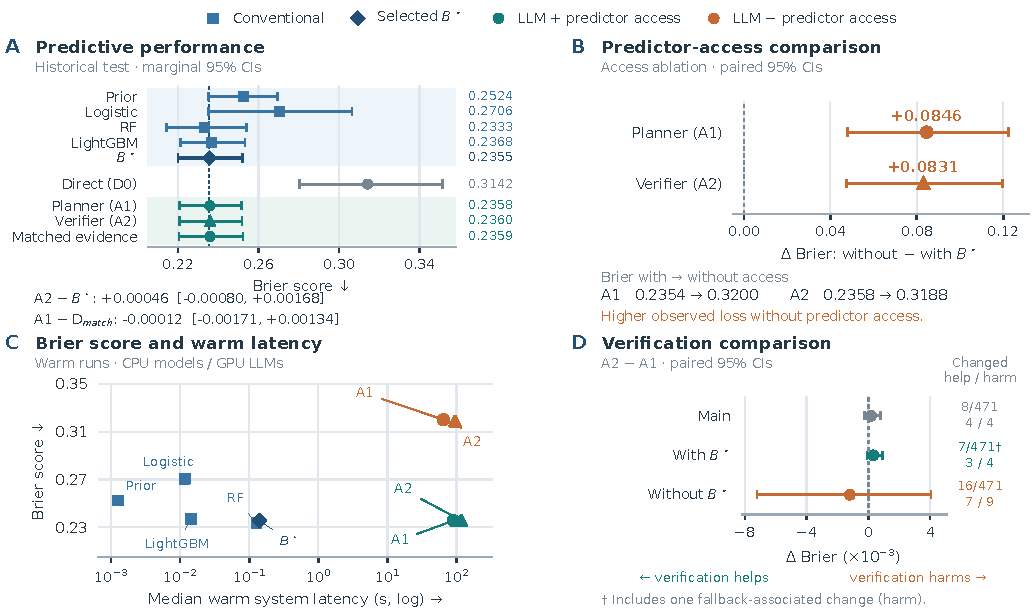
\includegraphics[width=\textwidth]{figures/results.pdf}
\caption{Exploratory comparisons on the previously examined 157 requests / 120 questions. A: main comparison; paired contrasts below. B: predictor-access ablation. C: packet-inclusive warm latency, including tools, verification and retries; CPU conventional models versus four RTX 4090 GPUs for LLMs (concurrency eight). Initialization and offline replay are separate. D: paired loss differences with and without verification; counts include repeated outputs and one marked fallback. Circles / triangles denote A1 / A2 in B--C. All intervals are question-cluster 95\% CIs; LLM scores average per-repeat losses and retain fallbacks.}
\Description{Panel A groups conventional predictors, direct LLM inference and tool-assisted methods with Brier intervals. Panel B shows positive paired increases in loss when predictor access is removed. Panel C compares all five measured conventional models with the four access-ablation systems using warm latency on a logarithmic axis. Panel D shows paired verification effects crossing zero, with changed-output and help-versus-harm counts alongside.}
\label{fig:results}
\end{figure*}

\section{Evaluation and results}
Our proper probability score~\cite{gneiting2007} and paired difference are
\begin{equation}
\widehat{\mathrm{BS}}_m=\frac1N\sum_i\frac1{R_m}\sum_r(p_{imr}-Y_i)^2,
\qquad\widehat\Delta_m=\widehat{\mathrm{BS}}_m-\widehat{\mathrm{BS}}_{B^\star}.
\end{equation}
Losses, rather than probabilities, are averaged across repeats; $N=157$, not 471. We jointly resample the 120 question clusters 9,999 times, using each draw's actual request count. Percentile 95\% intervals are marginal and conditional on these fits and runs. A null-centered studentized cluster bootstrap~\cite{cameron2015} gives $p=.4773$ for the original primary A2--$B^\star$ comparison. A degenerate draw in A2--A1 suppresses its $p$-value and the prespecified secondary Holm family~\cite{holm1979}; no new confirmatory tests are claimed for the access ablation.

\begin{table}[t]
\caption{Exact test estimates. $N=157$, $G=120$; $R=1$ for $B^\star$, otherwise 3. Paired question-cluster 95\% CIs. Bottom four rows are fresh access-ablation runs; all differences use the same frozen $B^\star$.}
\label{tab:exact}\centering\small
\begin{tabular}{@{}lrr@{}}
\toprule
System & Brier & $\Delta$ vs. $B^\star$ [95\% CI] \\
\midrule
$B^\star$ & 0.2355 & reference \\
D0 & 0.3142 & $+0.0787\ [+0.0428,+0.1168]$ \\
A1 & 0.2358 & $+0.0003\ [-0.0013,+0.0017]$ \\
A2 & 0.2360 & $+0.0005\ [-0.0008,+0.0017]$ \\
D$_{match}$ & 0.2359 & $+0.0004\ [-0.0003,+0.0011]$ \\
\midrule
A1, with $B^\star$ & 0.2354 & $-0.0001\ [-0.0016,+0.0013]$ \\
A2, with $B^\star$ & 0.2358 & $+0.0002\ [-0.0011,+0.0015]$ \\
A1, no $B^\star$ & 0.3200 & $+0.0845\ [+0.0479,+0.1227]$ \\
A2, no $B^\star$ & 0.3188 & $+0.0833\ [+0.0476,+0.1202]$ \\
\bottomrule
\end{tabular}

\end{table}

\paragraph{Attribution.}
Original A1 improves on D0 by $-0.0784$ Brier ($[-0.1167,-0.0425]$), but A1--D$_{match}$ is $-0.0001$ ($[-0.0017,0.0013]$). A2--$B^\star$ is $+0.0005$ ($[-0.0008,0.0017]$). All 471 original A1 trajectories call the predictor. These comparisons alone cannot attribute the gain to planning. \AblationFinding{}

\paragraph{Verification and dependence.}
In the original run, verification changes 8/471 predictions on eight requests: four improve and four worsen, yielding A2--A1 $+0.00018$ ($[-0.00024,0.00077]$). All eight move toward $B^\star$; the verifier's alleged errors are not independently established factual errors. \VerificationFinding{} Calendar sensitivity coalesces 7/14/28-day bins crossed by a whole question into 24/16/10 blocks; all original primary intervals include zero. \TemporalFinding{} Few blocks and possible shared events across questions limit inference.

\paragraph{Execution and costs.}
Original inference used 2,854 physical calls; 13 timeouts recovered on retry, with no fallback outputs. \ExecutionFinding{} Method-equivalent costs include their shared A1 prefix; physical ledgers count it once. Original median A2 latency is 185.87\,s versus 0.136\,s for $B^\star$, excluding initialization and packet construction. Fresh timing in Figure~\ref{fig:results}C includes packet construction from cached admissible features; offline event replay and initialization are separate. \PreparationFinding{} No dollar tariff or GPU-utilization estimate is invented. Training search took 17.62\,s on CPU; model loading and failed-call token uncertainty are recorded separately.

\section{Limitations and conclusion}
This selected settled cohort cannot estimate all-request deployment risk or external truth. The small search, one LLM, unknown pretraining cutoff and prior test exposure limit generalization. Read-only tools do not test general agent autonomy. Historical event replay is not independent receipt verification. The backup runtime's batching can change seeded draws, so reruns need not be bit-identical. An earlier outage run and a train-only preprocessing correction are preserved in the execution record. Saved probabilities, prompts, traces, scripts and figure sources accompany the local materials; external reviewer access remains to be arranged. \ConclusionAblation{} A confidence interval spanning zero does not establish equivalence. Prospective data and broader predictors are needed before deployment claims.

\balance
\bibliographystyle{ACM-Reference-Format}
\bibliography{references}
\end{document}
